\begin{center}
	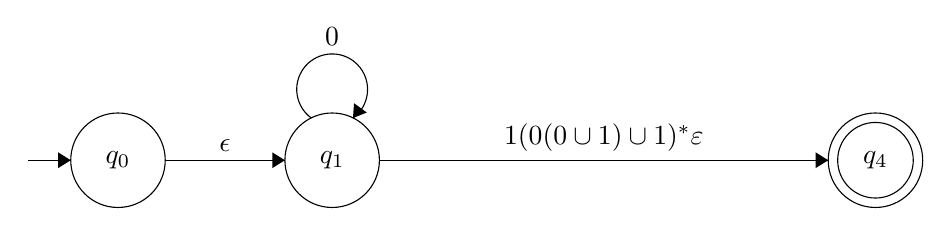
\begin{tikzpicture}[scale=0.2]
		\tikzstyle{every node}+=[inner sep=0pt]
		\draw [black] (30.1,-17.2) circle (3);
		\draw (30.1,-17.2) node {$q_1$};
		\draw [black] (16.5,-17.2) circle (3);
		\draw (16.5,-17.2) node {$q_0$};
		\draw [black] (64.6,-17.2) circle (3);
		\draw (64.6,-17.2) node {$q_4$};
		\draw [black] (64.6,-17.2) circle (2.4);
		\draw [black] (28.777,-14.52) arc (234:-54:2.25);
		\draw (30.1,-9.95) node [above] {$0$};
		\fill [black] (31.42,-14.52) -- (32.3,-14.17) -- (31.49,-13.58);
		\draw [black] (19.5,-17.2) -- (27.1,-17.2);
		\fill [black] (27.1,-17.2) -- (26.3,-16.7) -- (26.3,-17.7);
		\draw (23.3,-16.7) node [above] {$\epsilon$};
		\draw [black] (10.8,-17.2) -- (13.5,-17.2);
		\fill [black] (13.5,-17.2) -- (12.7,-16.7) -- (12.7,-17.7);
		\draw [black] (33.1,-17.2) -- (61.6,-17.2);
		\fill [black] (61.6,-17.2) -- (60.8,-16.7) -- (60.8,-17.7);
		\draw (47.35,-16.7) node [above] {$1(0(0\cup1)\cup1)^*\varepsilon$};
	\end{tikzpicture}
\end{center}
